\chapter{Serveur}

Ce projet a pour but de fournir un programme permettant de concevoir des bases d'apprentissage automatiquement pour l'entraînement de systèmes de reconnaissance d'écriture manuscrite. Il sera notamment exploité par les \href{http://archives.ille-et-vilaine.fr/fr}{archives d'Ille-et-Vilaine} ainsi que la startup \href{http://www.doptim.eu}{Doptim}. Les reconnaisseurs utilisés pouvant être multiples, il faut que ce projet puisse facilement évoluer, qu'une partie du projet puisse être remplacée par un morceau plus adapté au reconnaisseur choisi. Ainsi, tous les modules de notre projet et non seulement l'interface avec le reconnaisseur doivent pouvoir être remplacés par l'implémentation choisie par l'utilisateur. Par exemple, nous avons choisi une base de données intégrée avec \textit{SQLite} mais celle-ci ne peut gérer facilement l'accès concurrentiel, ou gérer efficacement une grande quantité de données. Ainsi, l'utilisateur pourrait choisir d'utiliser une autre base de données comme \textit{MySQL} ou \textit{MongoDB}. Nous avons donc dû prendre en compte dans l'architecture l'aspect interchangeable de nos modules. Notre \textit{back-end} est, nous le rappelons, écrit en Scala, et utilise des bibliothèques externes pour la gestion du JSON et des images (OpenCV par exemple). Nous utiliserons un serveur basé sur \href{https://javaee.github.io/grizzly}{\texttt{Grizzly}}, une technologie utilisée dans un projet précédent cette année, et qui nous a paru simple d'utilisation, ainsi que \href{https://jersey.github.io}{\texttt{Jersey}} pour l'API REST, pour les mêmes raisons.

\section{Architecture générale}

Le serveur de ce projet est composé de trois principaux modules représentant les différents besoins du projet. Ainsi, il nous faut traiter les données d'entrée fournies par l'utilisateur sous la forme d'un document scanné et possiblement d'une vérité terrain afin de les transformer en données utilisables par les reconnaisseurs. Il nous faut également pouvoir stocker les bases d'apprentissage qui constituent le coeur de notre projet. Enfin, ces bases ne serviraient à rien s'il n'était pas possible d'interfacer notre projet avec le reconnaisseur de l'utilisateur.

Notre projet étant composé de parties bien distinctes, la mise en place de modules indépendants et pouvant être remplacés par l'utilisateur n'a donc pas posé de problème. Nous avons donc créé une structure constituée des différents \textit{packages} correspondant aux fonctionnalités ainsi qu'une interface faisant le lien entre tous. De cette manière, chaque partie est détachée de l'ensemble global, et l'interface centrale qu'on appellera \texttt{Controller} fera appel aux méthodes nécessaires des différents \textit{packages}, afin de répondre aux demandes de l'utilisateur. Les \textit{packages} auront alors une interface à implémenter permettant une utilisation indépendante de l'implémentation.
\newpage
\begin{mdframed}[frametitle={Architecture des modules avec le connecteur}, innerbottommargin=10]
\begin{center}
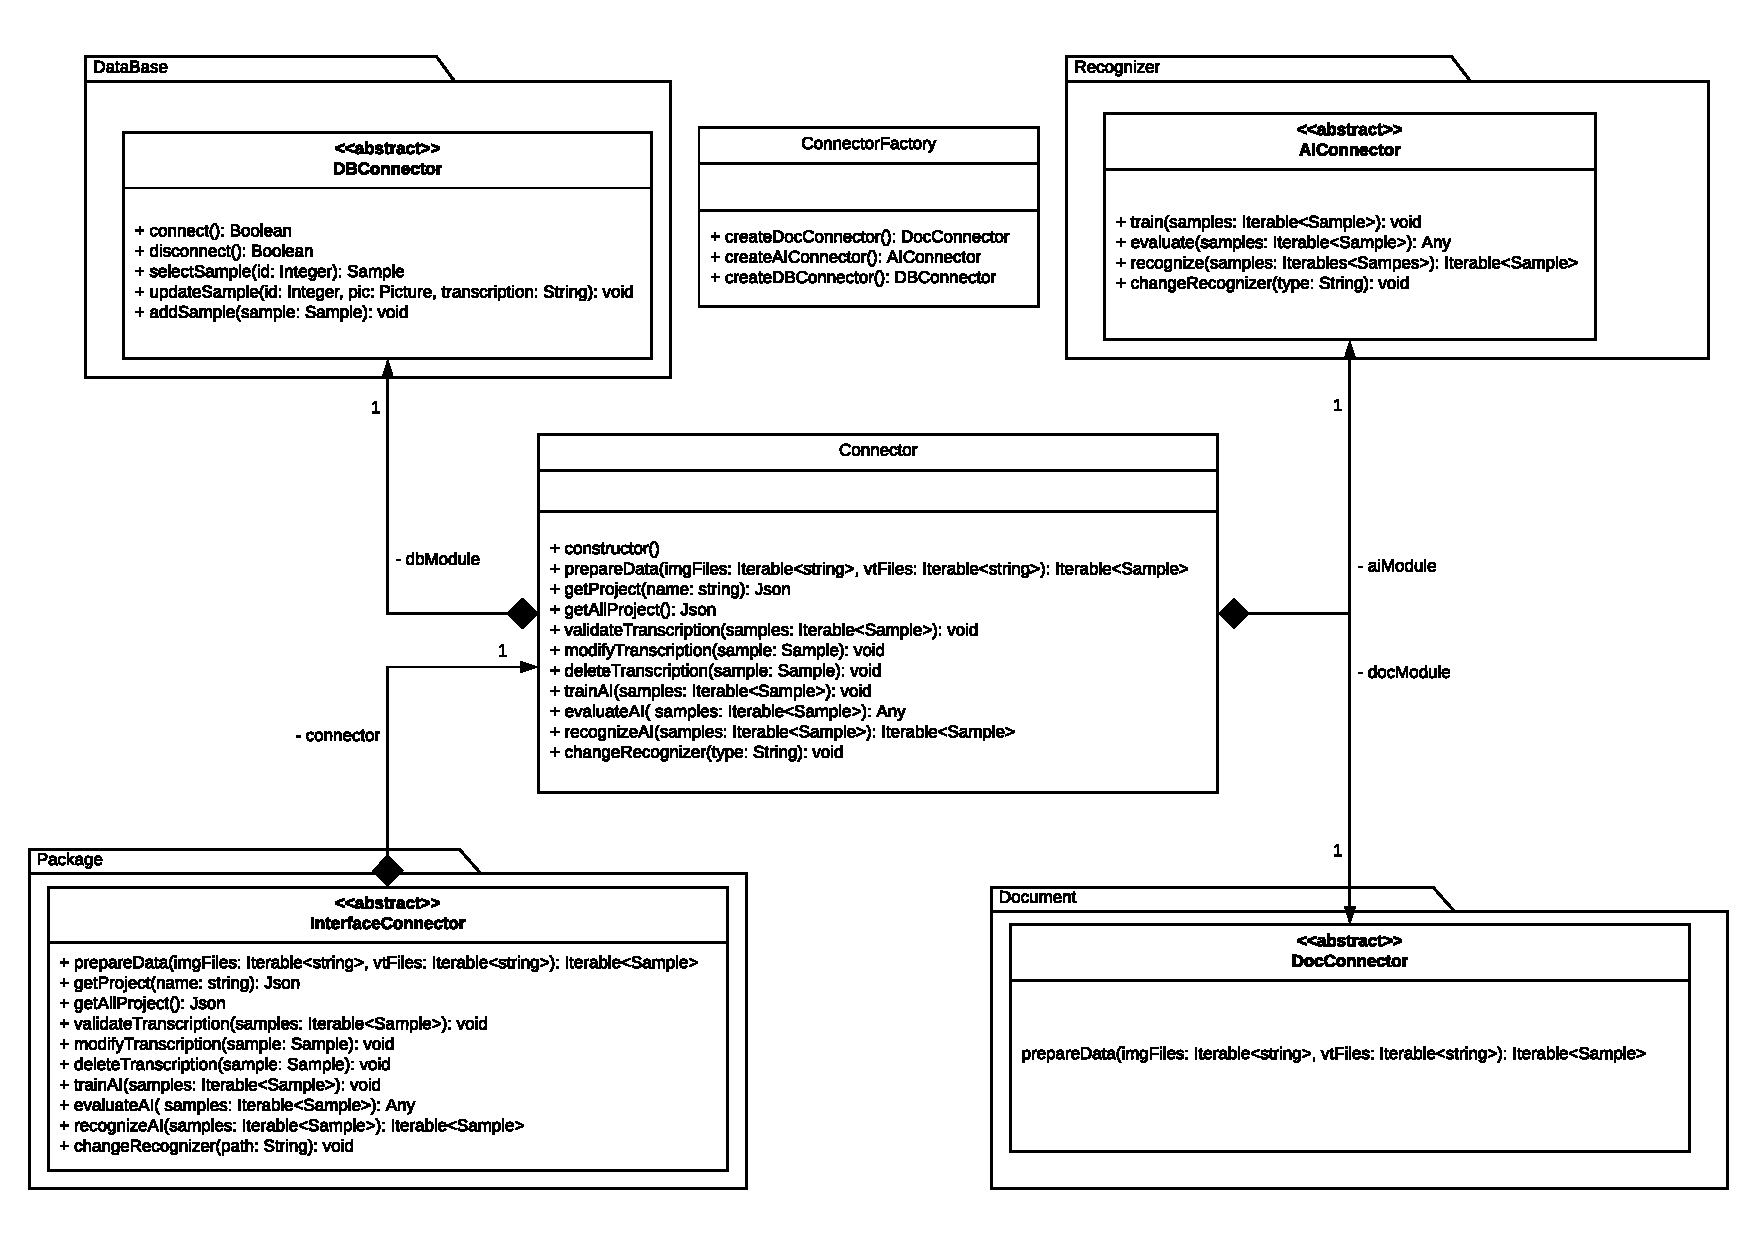
\includegraphics[trim={10cm, 0, 6cm, 0} ,scale=0.25]{assets/UML_connecteur.pdf}
\end{center}
\end{mdframed}

\paragraph{}
Dans notre projet, nous aurons également besoin de représenter les objets avec lesquels nous travaillons. Ainsi, nous avons choisi d'implémenter des classes de données pour représenter les exemples d'apprentissage (\texttt{Example}), les pages des documents utilisés (\texttt{Page}), lesdits documents (\texttt{Document}) et enfin les projets (\texttt{Project}) car on peut imaginer que l'utilisateur puisse vouloir avoir un projet sur des archives paroissiales et un autre sur des textes arabes anciens.

\begin{mdframed}[frametitle={Structure du package de données}, innerbottommargin=10]
\begin{center}
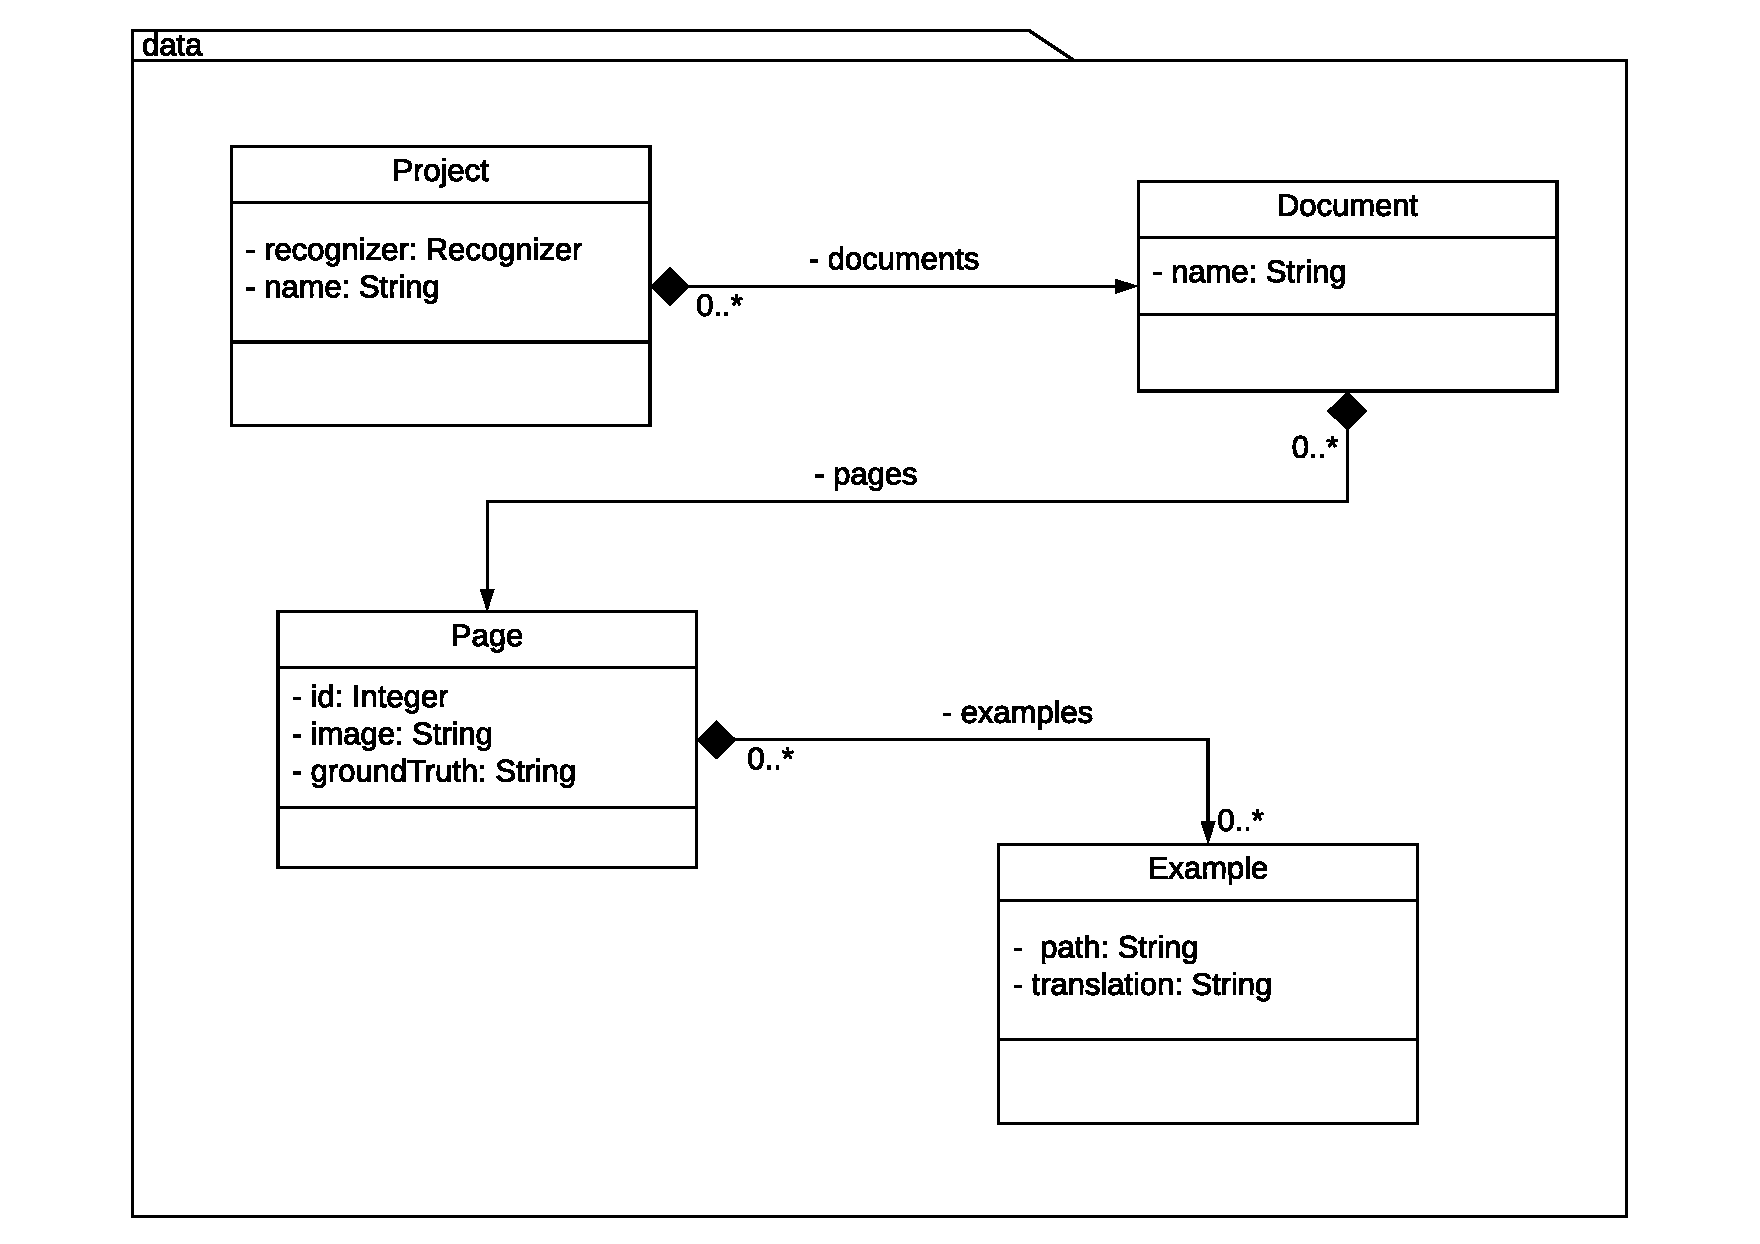
\includegraphics[scale=0.4]{assets/UML_data.pdf}
\end{center}
\end{mdframed}

L'attribut \texttt{Recogniser} est converti en \texttt{String} dans la base de données en passant par un \textit{enum} recensant les différents reconnaisseurs existants. Ces classes de données sont liées à la structure de la base de données et seront donc expliquées plus profondément dans cette partie.


%-----------------------------------------------------------------------------------------------------------------------
\section{Traitement des données}

Pour ce qui est du traitement des données, il nous faut un \textit{package} pour chacune des deux tâches concernées, à savoir la lecture des fichiers d'entrée ainsi que la découpe d'image.

\subsection{Lecture des fichiers d'entrée : \textit{package} \texttt{input}}

Comme expliqué dans le dernier rapport, nous avons choisi de ne traiter qu'un seul format dans notre logiciel, le format PiFF. Pour pouvoir lire les fichiers d'entrée, on doit construire une représentation des données contenues dans ces derniers sous la forme d'objets. Ceci constituera le \textit{package} \texttt{piff}. Il définit une classe \texttt{PiFF}, qui contient des pages (\texttt{PiFFPage}), qui elles-mêmes contiennent des portions de texte (\texttt{PiFFElement}). Ces classes peuvent être converties au format JSON (bibliothèque \href{https://mvnrepository.com/artifact/org.json/json}{org.json}), ce qui permet d'exporter les objets vers un fichier PiFF afin de répondre à la spécification \textit{PR\_F0\_1} pour l'utilisation du format PiFF en interne.

\paragraph{}
L'utilisateur doit toutefois pouvoir utiliser d'autres formats afin de permettre l'évolution de notre logiciel comme spécifié dans les précédents rapports (\textit{GEN\_EVO}). Pour cette raison, nous avons un \textit{package} \texttt{converters} contenant une interface, \texttt{PiFFConverter}, qui permet de convertir un fichier quelconque en objet \texttt{PiFF}. Nous en fournissons une implémentation, l'objet \texttt{GEDIToPiFFConverter}, qui comme précisé dans les précédents rapports (\textit{PR\_FO\_2}), permet au logiciel de lire le format GEDI. Celui-ci est utilisé notamment par la base de données Maurdor, présentée dans les précédents rapports, et à laquelle nous avons accès pour nos tests. L'utilisateur peut rajouter autant d'implémentations qu'il le souhaite.

\paragraph{}
En plus de ces deux \textit{packages}, nous proposons un objet \texttt{PiFFReader} (singleton), qui permettra d'ouvrir un fichier, et d'utiliser les concepts présentés ci-dessus. Plus précisément, il permettra de lister des implémentations de \texttt{PiFFConverter}, et de les appeler une par une sur le fichier d'entrée pour réussir à le lire.

\subsection{Découpe des images : \textit{package} \texttt{processing}}

Pour la découpe d'image, il nous faut une classe \texttt{ImageProcessing}, qui appelle les méthodes de la bibliothèque OpenCV, que nous avons choisie précédemment. Cette bibliothèque nous permet de découper les images afin d'obtenir les imagettes selon les lignes ou les paragraphes (\textit{PR\_TR\_2 et PR\_TR\_4}). Après la découpe, les imagettes sont associées au texte pour former des exemples, que nous avons modélisés par une classe \texttt{Example} (spécifications \textit{PR\_RE\_1 et PR\_RE\_2}). 

\paragraph{}
La phase de découpe étant automatique, il nous faut faire appel à un détecteur de lignes. C'est la fonction du \textit{package} \texttt{linedetection}. Nous y plaçons une interface \texttt{LineDetector}, qui permet de trouver les lignes de texte dans un objet PiFF (spécification \textit{PR\_TR\_1}). Le détecteur de lignes utilisé pour le projet est fourni par l'encadrant, et fonctionne sous Linux. Les membres du groupe peuvent pourtant travailler sous Windows ou macOS. Pour faciliter le développement du logiciel, nous avons donc choisi de fournir une implémentation, la classe \texttt{BlurLineDetector} (nom dû à la méthode de détection), basée sur des connexions réseau, afin de pouvoir faire fonctionner le serveur sous n'importe quel système d'exploitation, avec un petit module serveur sous Linux qui appelle simplement l'exécutable. Ce petit module ne fait pas partie du cahier des charges mais sera développé pour les tests. L'utilisateur, ici aussi, pourra rajouter ses propres méthodes de détection de lignes s'il le souhaite.

\paragraph{Version}

%----------------------------------------------------------------------------------------------------------------------
\section{Base de données}

Le Système de Gestion de Bases de Données (SGBD) choisi est SQLite. La bibliothèque Java SQLite, une implémentation de l'API JDBC (Java DataBase Connectivity), nous servira à appeler des commandes SQL directement depuis notre programme.
Il nous faut cependant remanier les relations entre les tables de la base de données, car en nous concertant avec l'équipe à propos de l'ergonomie à apporter ainsi que de la forme que devaient prendre les données, nous avons remarqué que notre précédente organisation ne pouvait fournir tous les éléments nécessaires. En effet, dans les précédents rapports, la forme que devait prendre l'IHM quand aux données venant du serveur et dont elle aurait besoin était plutôt floue. C'est en se penchant plus en avant lors de ce rapport que nous l'avons remarqué.

\subsection{Architecture}

La nouvelle base de données se base sur les classes de données présentées dans la première partie. Elles sont donc composées d'une table \texttt{Projects} qui contient les projets existants ainsi que le \texttt{Recogniser} associé. Celui-ci est représenté sous la forme d'une chaîne de caractères car un \textit{enum} sera mis en place afin de constituer les différents reconnaisseurs possibles et qu'on peut restorer l'\textit{enum} facilement à partir d'une chaîne de caractères. Une autre table \texttt{Documents} représente les différents documents qui constituent notre base, par exemple, \textit{"Archives paroissiales de 1870-1872"}. Ceux-ci sont donc représentés par un nom et sont liés à un \texttt{Project}. Une troisième table nous permet de conserver les \texttt{Pages} des \texttt{Documents}. Elles sont donc liées à une image (le scan de la page) et à une vérité terrain (la description de l'image) qui sont stockées au travers de leur chemin dans le système de fichier pour les raisons expliquées dans les rapports précédents (\textit{STO\_VER}). Les \texttt{Pages} sont également associées au \texttt{Document} dont elles sont issues. Enfin, une dernière table \texttt{Examples} stocke les \textit{exemples} générés par la découpe. Ils sont constitués du chemin vers l'imagette correspondante ainsi que la transcription de celle-ci, sachant que cette transcription peut être nulle dans le cas où on souhaite utiliser le \textit{reconnaisseur} pour proposer une transcription (\textit{STO\_REC}), ou quand la vérité terrain n'a pas été fournie et qu'il faut la construire (\textit{STO\_USR}). Les \texttt{Examples} sont également liés à la \texttt{Page} d'où ils ont été découpés.

\begin{mdframed}[frametitle={Structure de la base de données}, innerbottommargin=10]
\begin{center}
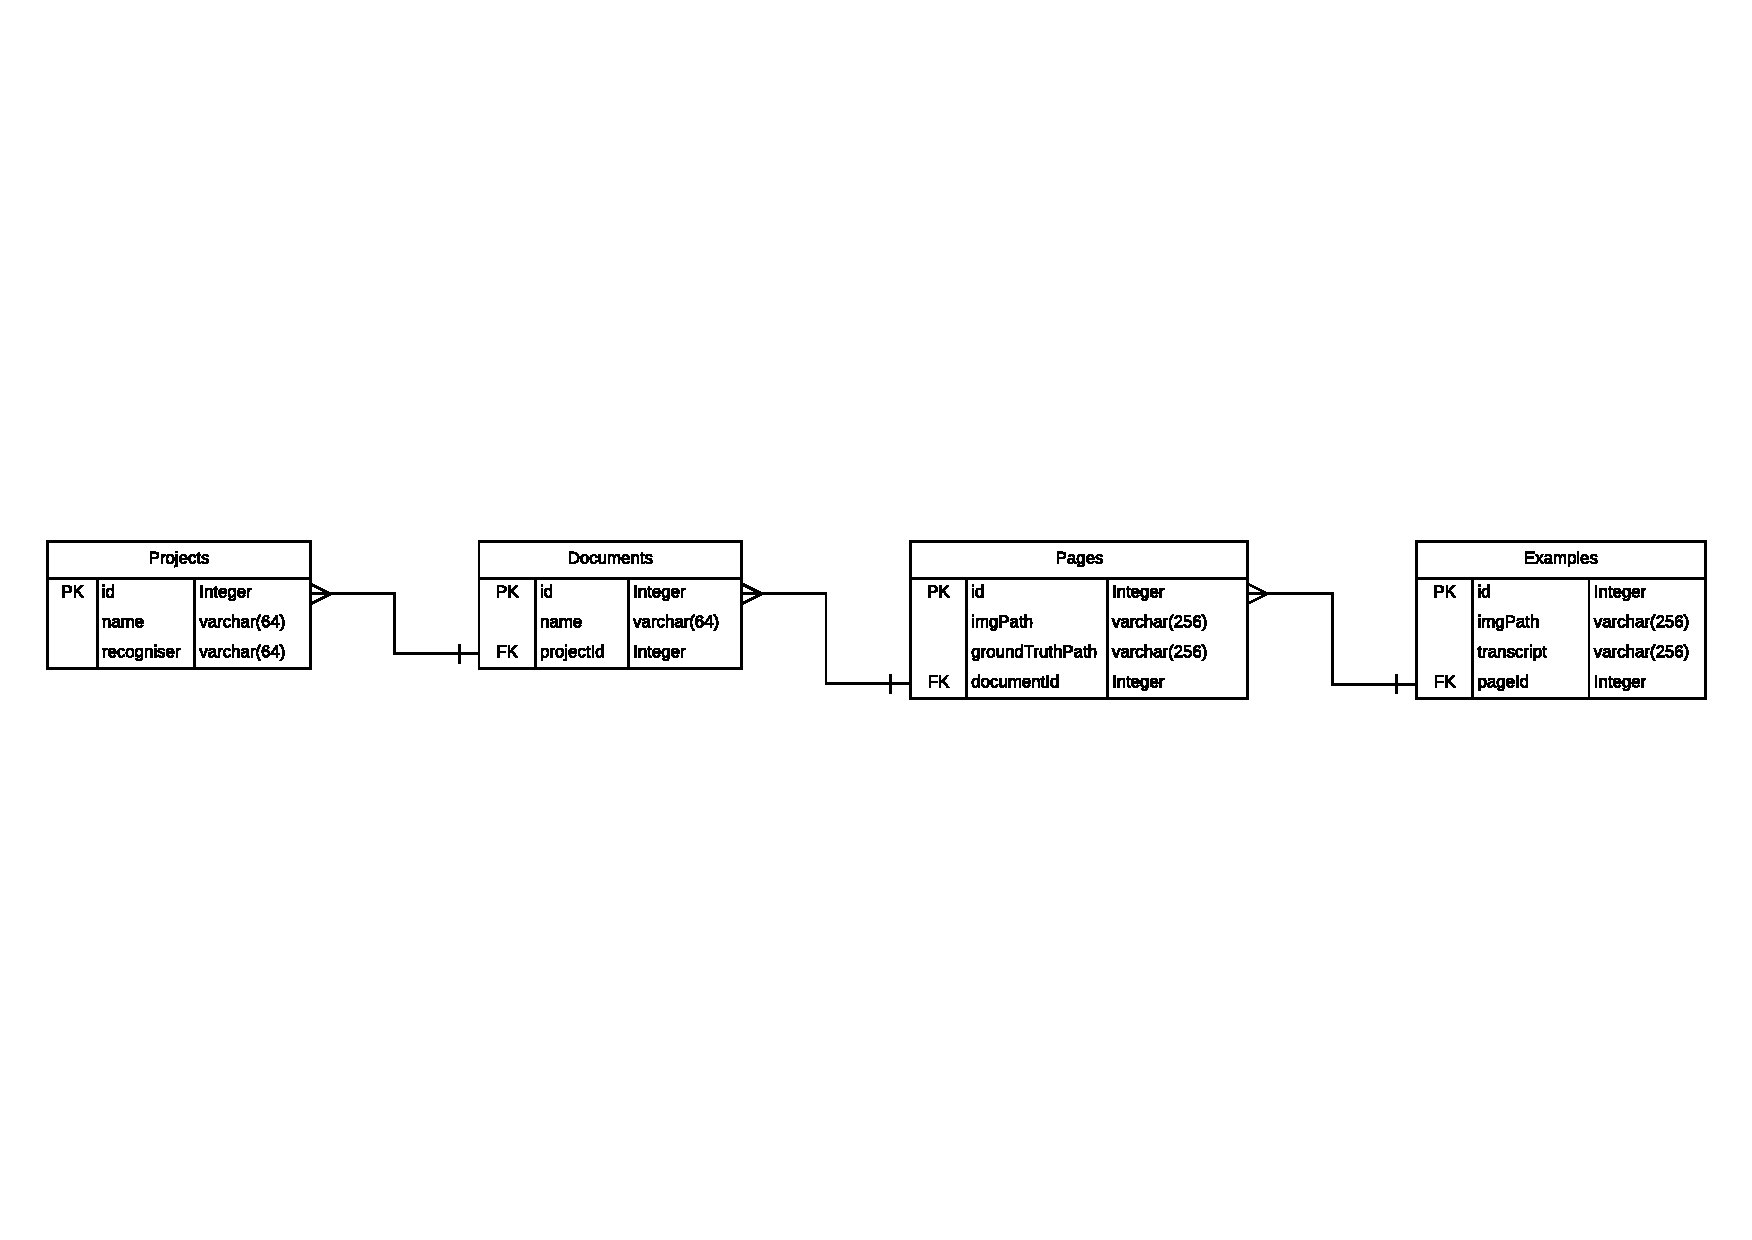
\includegraphics[scale=0.53]{assets/DatabaseEntity.pdf}
\end{center}
\end{mdframed}

Cette structuration nous permet de hiérarchiser les exemples d'apprentissage générés par notre logiciel et donc de pouvoir fournir une plus grande ergonomie au sein de l'application client.

Le module de la base de données est constitué d'une interface représentant cette base de données ainsi que les opérations qui seront effectuées dessus (\textit{STO\_SEL, STO\_UPD, STO\_INS, STO\_DEL}). Ainsi, il est possible de récupérer les différents instances de la hiérarchie de données. Nous avons préféré garder les requêtes sur la base de données simples et élémentaires afin de permettre plus de flexibilité sur les opérations qui les utiliseront ensuite. De cette manière, plusieurs fonctions du \texttt{Controller} pourront appeler la même fonction dans la base plutôt que d'avoir des demandes précises sur la base de données. De cette manière, l'évolution du projet en est simplifiée en permettant l'établissement simple de nouvelles fonctions dans le \texttt{Controller} sans avoir à rajouter de requêtes dans la base de données.

\newpage
\begin{mdframed}[frametitle={Architecture de la base de données}, innerbottommargin=10]
\begin{center}
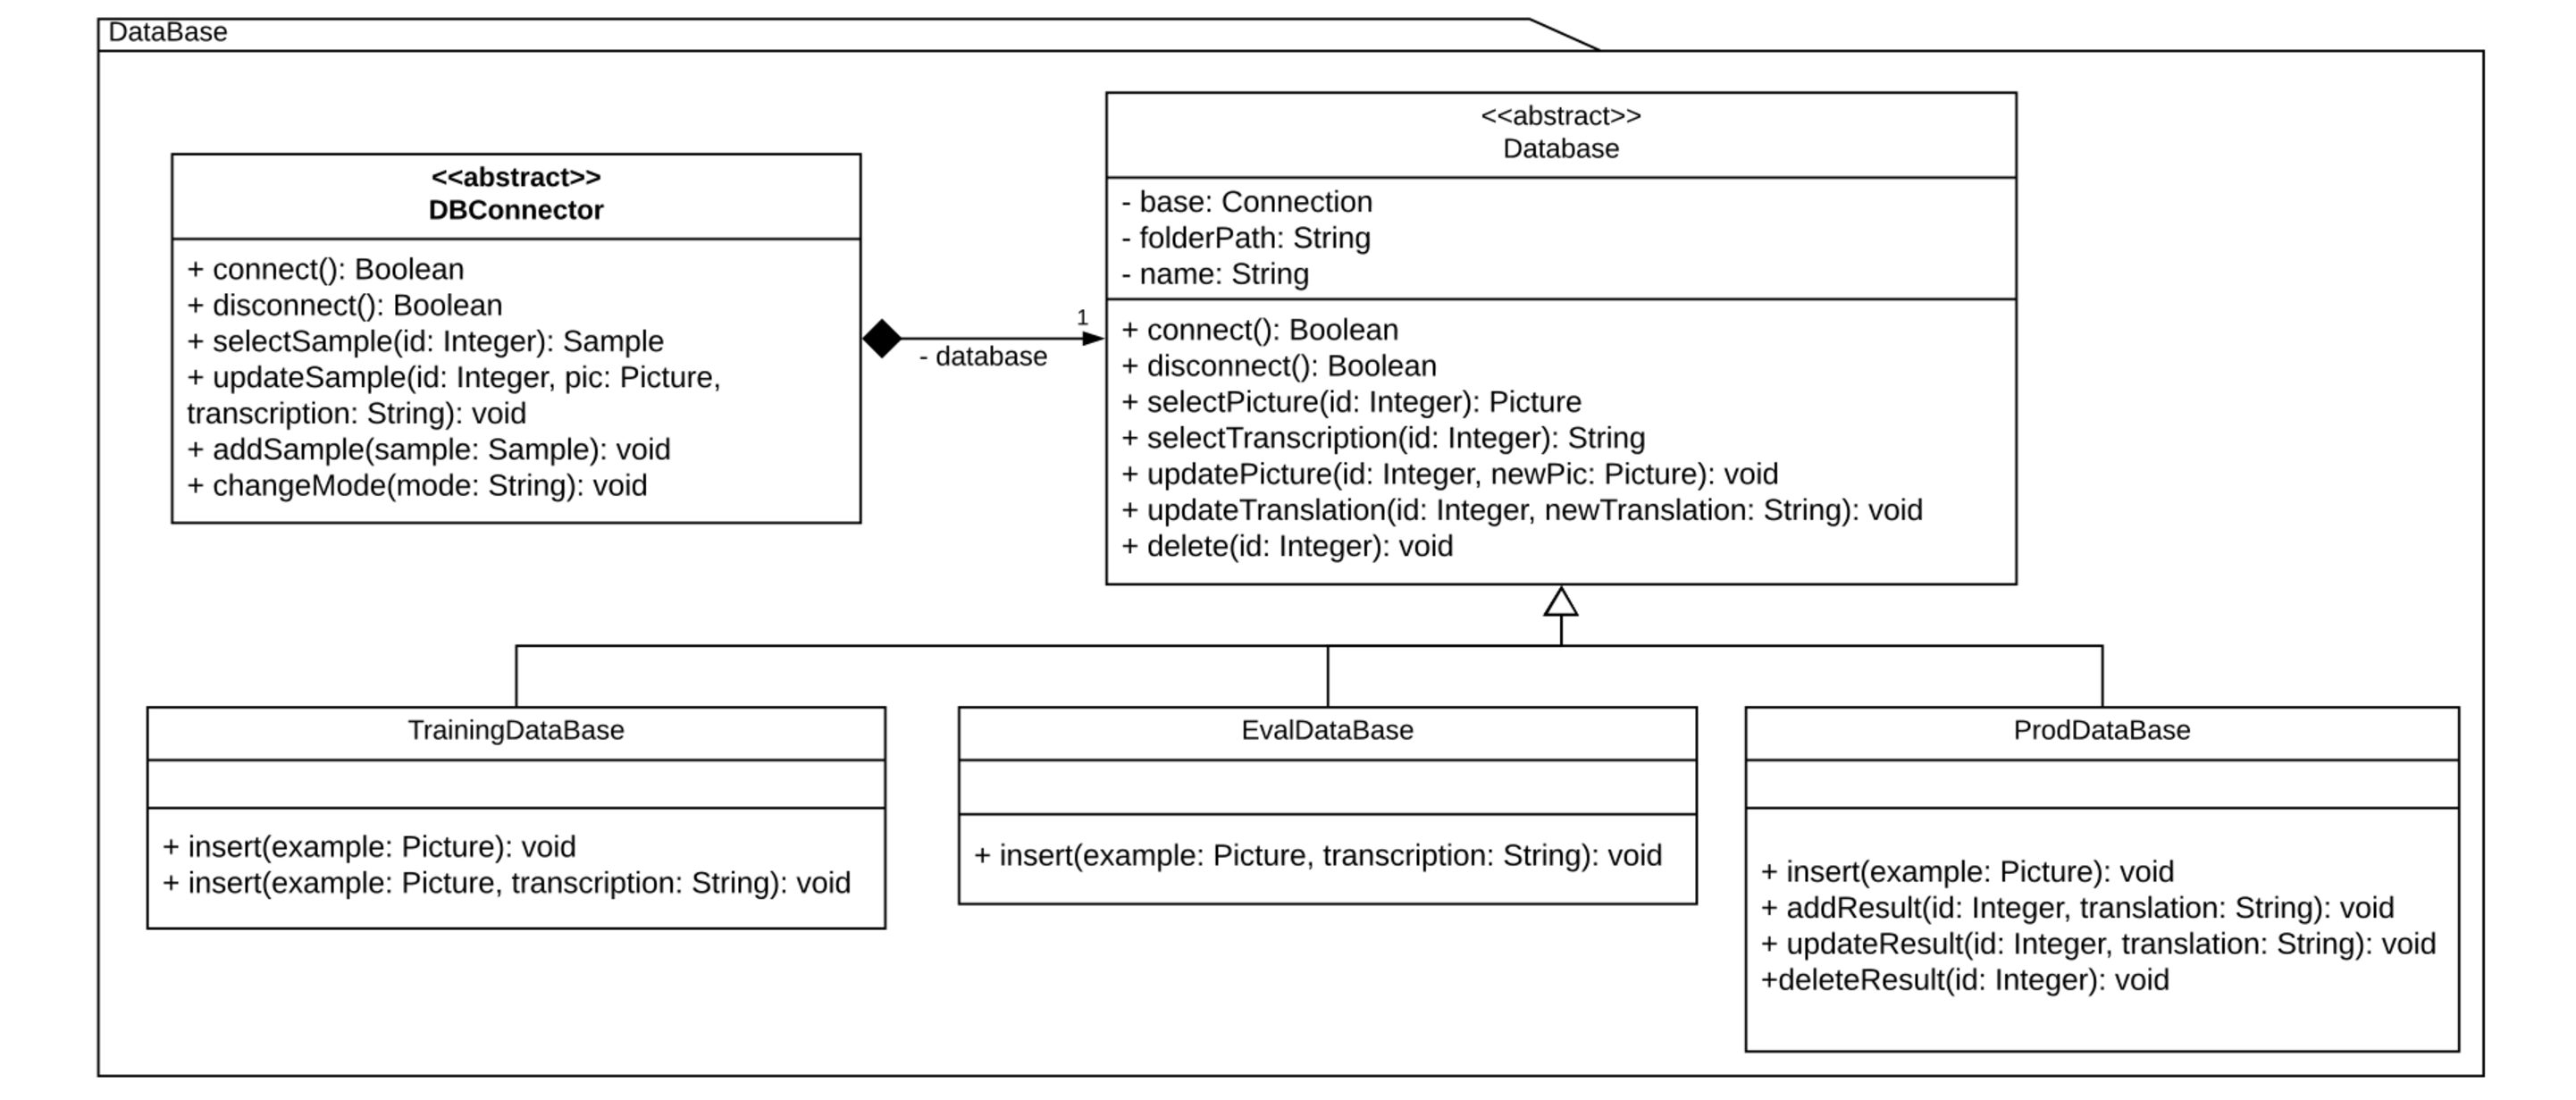
\includegraphics[scale=0.5]{assets/UML_Database.pdf}
\end{center}
\end{mdframed}

\paragraph{Version}
Comme l'ensemble des méthodes de la base de données sont nécessaires pour les appels de l'API REST, toute la classe devra être implémentée. L'ensemble des tables qu'elle manipule seront aussi créées. Pour la seconde itération de notre projet, de nouvelles méthodes ne seront pas nécessaires comme nous réutiliserons celles déjà créées pour les ajouts de méthodes dans le \texttt{contrôleur}. En revanche, pour cette seconde partie, le serveur et le client pouvant être sur des machines distinctes, nous devrons envisager un envoi des images au client, et non pas seulement des chemins de fichiers. La solution technique exacte n'est pas encore fixée, nous y réfléchissons en se basant sur les conseils de nos encadrants, qui ont eu des situations similaires dans leurs projets professionnels.

%-----------------------------------------------------------------------------------------------------------------------
\section{Interface avec le reconnaisseur}

Cette partie du projet a pour objectif de lier la base d'apprentissage de notre logiciel avec le reconnaisseur choisi par l'utilisateur. Ainsi, cette partie étant très liée à l'utilisateur, il faut lui permettre de pouvoir facilement attacher le reconnaisseur de son choix au logiciel. C'est avec cette contrainte en tête que nous avons conçu l'architecture de cette partie.

\begin{mdframed}[frametitle={Architecture de l'interface avec le reconnaisseur}, innerbottommargin=10]
\begin{center}
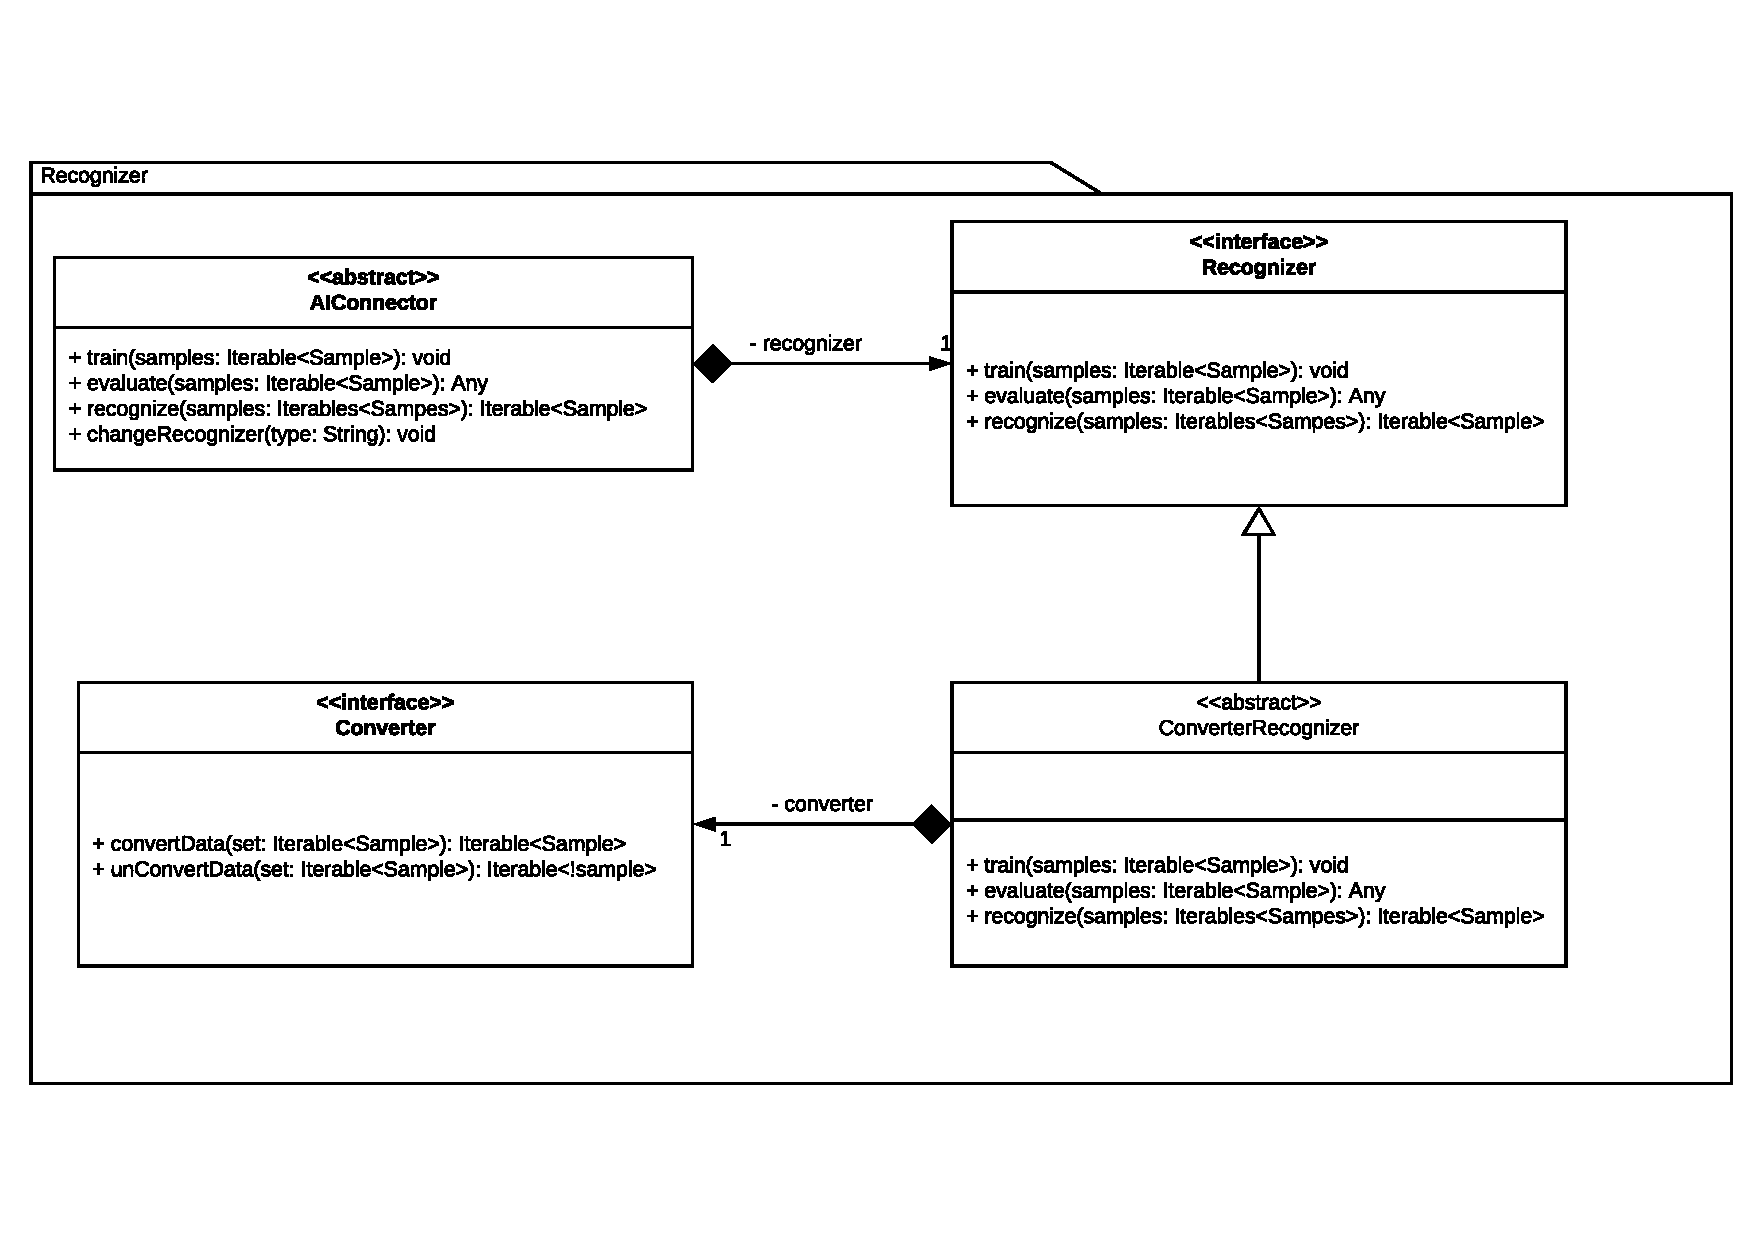
\includegraphics[trim={0, 0, 0, 0}, scale=0.55]{assets/UML_Recognizer.pdf}
\end{center}
\end{mdframed}

\paragraph{Architecture}

Cette partie du projet contient comme toutes les autres un connecteur qui la lie au \texttt{Connector} principal. Ce connecteur possède un \texttt{Recogniser} afin de pouvoir effectuer les opérations classiques d'entraînement, d'évaluation de celui-ci ainsi que lui demander d'effectuer une transcription. Il permet également de changer de reconnaisseur quand l'utilisateur souhaite utiliser un autre type de reconnaisseur.
\newline{}
Le reconnaisseur est représenté par une interface \texttt{Recogniser} qui permet trois actions possibles : entraîner le reconnaisseur à partir d'un ensemble d'apprentissage, évaluer ce même reconnaisseur sur un ensemble de validation, et enfin, lui demander de transcrire un ensemble non étiqueté. Ces fonctions ont été construites afin de répondre aux spécifications \textit{IR\_AP}, \textit{IR\_EV} ainsi que \textit{IR\_TR}.
Cette interface permet notamment à l'utilisateur de connecter son propre reconnaisseur, et même s'il le souhaite, d'en créer un au sein de l'application. Elle est également la seule qu'il est obligé d'implémenter pour faire fonctionner l'ensemble. Cependant, il faut dans certains cas convertir les données dans la base de données en données compréhensibles par le reconnaisseur. Ainsi, deux autres interfaces sont nécessaires : une interface \texttt{Converter} permettant la conversion des données entrantes et sortantes du reconnaisseur (\textit{IR\_CV}) ainsi qu'une classe abstraite \texttt{ConverterRecogniser} héritant de \texttt{Recogniser} et possédant un convertisseur adapté au reconnaisseur utilisé. En effet, le reconnaisseur peut avoir besoin d'un formatage des images en entrée, mais également de la transcription associée. Par exemple, nous implémenterons la structure décrite précédemment pour un reconnaisseur particulier : \href{https://github.com/jpuigcerver/Laia}{Laia}. Ce reconnaisseur demande de transformer les images afin qu'elles aient la même hauteur en pixels, et que la transcription soit traduite dans les symboles qu'il peut reconnaître et organisée d'une certaine façon. Par exemple, il faut remplacer les ' ' par '<space>' et que l'identifiant de l'image correspondante à la transcription soit indiqué avant celle-ci dans un fichier. Le convertisseur va donc se charger de mettre en forme les données et de créer ce qui est nécessaire.
\paragraph{Version}
Dans la première version délivrée le 27 Février, la possibilité d'entraîner le reconnaisseur doit être implémentée ainsi que celle de changer de reconnaisseur. Dans un second temps, il sera possible de faire transcrire les imagettes par le reconnaisseur et de faire l'évaluation de celui-ci. Les données remontées lors de l'évaluation sont laissées libres à l'utilisateur puis la fonction rend un objet non défini à l'avance qui sera sous la forme d'un \textit{JSON} et qui contiendra les informations choisies par l'utilisateur dans son implémentation. Il pourra alors obtenir le nombre et la fréquence des erreurs, sur quelles lettres celles-ci surviennent et ainsi de suite.

%----------------------------------------------------------------------------------------------------------

\section{Contrôleur}
\subsection{Architecture}

Le rôle du contrôleur est de mettre en relation les 4 parties du projet : le \textit{client}, \textit{i.e.} l'interface homme-machine, la base de données, ainsi que le traitement des données. Pour ce faire, nous avons 4 classes abstraites, un connecteur par \textit{package} du projet, chacun possédant des méthodes générales, qui appellent d'autres méthodes de leurs \textit{packages} respectifs. Cela permet d'avoir un objet \texttt{Controller} central qui manipule tous les éléments du projet avec un code très lisible. Nous fournissons une implémentation de chaque connecteur, pour le bon fonctionnement du projet. Une fabrique est également prévue, permettant de choisir l'implémentation des connecteurs de chaque partie sans avoir à modifier le code du connecteur central. En effet, le contrôleur récupèrera les instances des connecteurs à partir de cette fabrique. Cela permet à l'utilisateur de changer d'instance de connecteur en changeant une ligne de code seulement.

Pour la première version de notre projet, le \texttt{Controller} devra permettre de relier les différents modules au travers de leurs interfaces de connection ainsi que permettre les exécutions des demandes en provenance de l'utilisateur, c'est à dire le client. 

\subsection{Interactions}
\paragraph{}
Le connecteur central reçoit donc, au travers du connecteur en relation avec le client les demandes de l'utilisateur et, afin d'exécuter ces demandes, appelle au travers des connecteurs des autres modules les méthodes nécessaires. Le \texttt{Controller} sert alors d'intermédiaire entre l'utilisateur et les différents modules. Il permet notamment cette structure modulaire en détachant les appels de méthodes des classes réelles qui peuvent alors être changées selon le bon vouloir de l'utilisateur.
